
\documentclass[10pt,sigconf, review]{article}
% \documentclass[sigconf,review]{acmart}

% \usepackage[british]
\usepackage[british]{babel}

\usepackage[letterpaper]{geometry}
\usepackage{hicss}
\usepackage{times}
\usepackage[none]{hyphenat}
\usepackage{url}
\usepackage{latexsym}
\usepackage{minted}
\usepackage{indentfirst}
\usepackage{graphicx}
\graphicspath{{images/}}

\newcommand{\sansserifformat}[1]{\fontfamily{cmss}{ #1}}%

\usepackage[hidelinks]{hyperref, xcolor}

\renewcommand\UrlFont{\color{blue}\rmfamily}

\setlength\titlebox{8cm}

% You can expand the titlebox if you need extra space
% to show all the authors. Please do not make the titlebox
% smaller than 5cm (the original size).


\title{ \huge A 2-Factor Authentication Safe System using Shape Recognition}

 % Comment this for initial manuscript 
 % Uncomment this for final manuscript

\author{BD Zwane \\
  \textbf{216446704}\\
  \em{Computer System Engineering}\\
  \em{Thswane University of Technology}\\
  \em{Pretoria, South Africa}\\

  \And

  SH Khoza \\
  \textbf{214651459}\\
  \em{Computer System Engineering}\\
  \em{Thswane University of Technology}\\
  \em{Pretoria, South Africa}\\

  \And 

  MM Cele \\
  \textbf{218243401}\\
  \em{Computer System Engineering}\\
  \em{Thswane University of Technology}\\
  \em{Pretoria, South Africa}\\}

\date{}


\begin{document}

\maketitle

\begin{abstract}

A safe is a secure lockable box used for securing valuable objects against
theft and/or damage from fire. However, keeping your valuables safe these days
is difficult even if you have a safe with security code people can always copy
it without your attention and access your belongings. The project adds a second
authentication mechanism to a safe that requires shape detection. The
implementation of object detection will improve the security or protection of
the safe by having to scan a randomly sent shape. The project will be
implemented using Raspberry Pi, Finite State Machine(FSM), shape detection will
be achieved by using Webcam and Python code.

Raspberry pi, Finite state machine, Multiplexers, detection algorithm
name, OpenCV

\end{abstract}

\section{Introduction}
 
According to \href{https://en.wikipedia.org/wiki/Crime_in_South_Africa}
{\color{blue}Wikipedia} South Africa has a notably high rate of murders,
assaults, rapes, and other violent crimes, compared to most countries. , that's why it is important to keep your money
extra safe. A safe box offers that safety, not only for money but other valuable
material such as jewelry nevertheless criminals still access the safe, we
believe shape recognition can improve the safety of the safe box.

Passwords used to be a created method to protect systems or devices, but with
the numbers of hackers or tools available today such as  attack it
\href{Brute-force} {\color{blue}Brute-force}, has become much easier to break
them. A second authentication method from password can prevent such
vulnerability of a protected device.
  
\href{https://link.springer.com/chapter/10.1007/978-3-642-23687-7_43}
{\color{blue}Sang Hwa LeeSiddharth SharmaLinlin SangJong-Il ParkYong Gyu Park},
published a paper title An Intelligent Video Security System Using Object Tracking and
Shape Recognition The proposed system integrates the object extraction, human
recognition, face detection, object tracking, and camera control.

Our system introduces a third level of authentication on the safe box, to make
sure if the owner is the one trying to access the box, first a user will enter
a password, then after they’ve entered a password an SMS will be sent to their
phone with a shape that is supposed to be scanned. Once they scan it then they
will be able to access the safe box

According to Businesstech, a report on 3 August 2019 a research was conducted
in 2016 and “based on in-depth interviews with convicted robbers they found
that 8 out of 10 residenti robberies are committed using information from
domestic workers, gardeners and former employees.” As a result, we assume that
the workers or employees may have once seen the codes to access things
including a safe in the house so out of fear of their threatened lives or at
some point the anger of unfair dismissal they give out the codes


\section{Background : related work}

Safe boxes are a reliable way to securely keep our most priced items and even
money, they are heavily dependent on a combination key(PIN) as security. As
much as it is not easy to break this combination key, having an extra-layer of
security is important to improve the security. Imagine a safe box with a
2-factor security system; that’s our project.

In South Africa, banks were offering it as a service to their select few
wealthy customers, however now the demand for safe boxes from banks has
significantly declined. This is because of the ``Safe box” heist that took
place in 2016 at an FNB branch in Gauteng, published by IOL  and 947. The
outcry was not about the robbery itself but about the bank saying it’s not
liable for the loss. This made people rely on keeping the safe boxes in their
private homes and/or private companies.

Petrol stations and supermarkets heavily rely on safe boxes to store money
while waiting for it to be collected for off-premises safekeeping. These are
the reasons we decided to add an extra layer of security to safe boxes.


\section{Specifications}

\begin{itemize}
  \item {One of the 4 USB port from the Raspberry Pi is going to be used to connect a Webcam}
  \item {A standard USB Webcam to scan/take pictures of shapes as input}
  \item {LCD screen will be used to display input messages e.g. enter a PIN code}
  \item {A user will be asked to enter/ key-in a PIN}
  \item {A 4x4 keypad will be used to key-in the safe box PIN}
  \item {An orange LED will indicate If the PIN is correct, else a red LED will indicate}
  \item {If a PIN is correct an MMS will be sent to the person who’s responsible in safe box stating which shape to be scanned}
  \item {A user will be asked to scan the shape that was stated via MMS}
  \item {A green LED will indicate If the shape is correct, else a red LED will indicate}
\end{itemize}

\section{Methods}

Finite State Machine - Our system will use the finite state machine approach as
we are executing steps sequentially until the final step.

Shape detection - The system will have a shape detection as a second step of verification. A randomly sent shape will be scanned using a webcam and compared with the one on the system.


\subsection{Operations of the project}

Explain all the algorithm that you are using here. List them as A, B C … (2 or
3 algorithms are enough.) Algorithm. Flow chart of your project can be put
here. You can use any software to draw it and copy the image here ( Please
don’t draw it with words )


% For one-column wide figures use
\begin{figure}[thb]
	% Use the relevant command to insert your figure file.
	% For example, with the graphicx package use
    \centering
	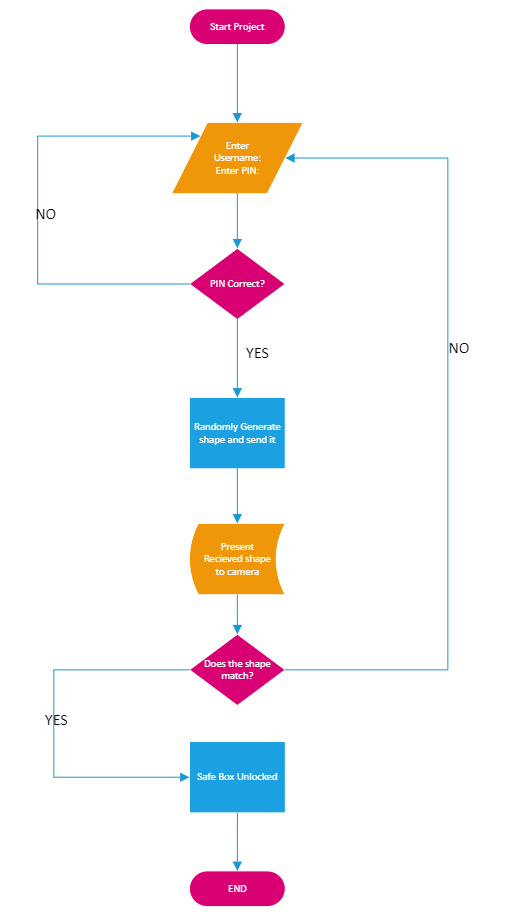
\includegraphics[trim={3cm 3cm 3cm 3cm}, clip,width=0.9\linewidth]{wor}
	% figure caption is below the figure
	\caption{Sample figure with caption.}
	\label{fig: sample-figure}       % Give a unique label
\end{figure}



\subsection{Algorithms}
Explain all the algorithm that you are using here. List them as A, B C … (2
algorithms are enough.) Algorithm/\\
Flow chart should be used to explain your algorithm.\\
After explaining the algorithm, you can summarize it as follow:\\

Algorithm 1:
\begin{enumerate}
	\item Start the project
	\item Upload the image 
	\item Check if the shape is recognized ?
  \item Does it match with any stored or acknowledge shape
  \item Give the output message
\end{enumerate}

This is just an example that I have made for you. You can customize it as you
want.

\subsection{Equations}
If you have equations in your report please type them using the recommendation below
The equations are an exception to the prescribed specifications of this
template. You will need to determine whether or not your equation should be
typed using either the Times New Roman or the Symbol font (please no other
font).


\section{Simualtions}
Here you can put figures or images of your software simulations, the outputs
waves of Quartus can be placed and explain each figure. Put some pictures of
your projects simulations, some LCD display output.

% For one-column wide figures use
\begin{figure}[thb]
	% Use the relevant command to insert your figure file.
	% For example, with the graphicx package use
    \centering
	
\includegraphics[trim={3cm 3cm 3cm 3cm}, clip,width=0.9\linewidth]{sample-image}
	% figure caption is below the figure
	\caption{Sample figure with caption.}
	\label{fig: sample-figure}       % Give a unique label
\end{figure}


Author names and affiliations must be included in the submitted Final Paper for
Publication. Leave two 12-point blank lines after the author’s information. 

\section{Second and following pages}
\label{sect:pdf}

The second and following pages should begin 1.0 inch (2.54 cm) from the top
edge. On all pages, the bottom margin should be 1-1/8 inches (2.86 cm) from the
bottom edge of the page for 8.5 x 11-inch paper. (Letter-size paper)

% \section{Type-style and fonts}


% \label{sec:type-style}
% Please note that {\em Times New Roman} is the preferred font for the text of
% you paper. \textbf{If you must use another font}, the following are considered
% base fonts.  You are encouraged to limit your font selections to Helvetica,
% Arial, and Symbol as needed. These fonts are automatically installed with the
% viewing software. 

\section{Discussions}
Discuss all the results of your projects Discuss what you have achieve and tell
us why it is important. Explain every output figure that you have. What it does
and how you understand it.

\section{Conclusion}
Conclude your paper efficiently by giving the overall statement of your
project. State what you have achieved and why it was important achieving. If
possible give 


\section{References} 

% The template will number citations consecutively within brackets [1]. The
% sentence punctuation follows the bracket [2]. Refer simply to the reference
% number, as in [3]—do not use “Ref. [3]” or “reference [3]” except at the
% beginning of a sentence: “Reference [3] was the first ...”

\begin{small}
    \begin{itemize}
      \item {Stacy Coley. (2019). Safe Deposit Boxes Aren\textquotesingle t
          Safe. The New York Times, [online]. Available at:
          \href{https://www.nytimes.com/2019/07/19/business/safe-deposit-box-theft.html}
        {\color{blue}www.nytimes.com}, [Accessed 22 Oct. 2020] }

      \item {John Doe. (215). Hole drilled by burglars at Hatton Garden
        revealed BBC News, [online]. Available at:
        \href{https://www.bbc.com/news/uk-england-london-32414531?ocid=socialflow_twitter}
      {\color{blue}www.bbc.com/news/}, [Accessed 23 Oct. 2020] }

      \item {Staff Writer. (215). FNB safety deposit box heist victims are
        suing for R121 million. businesstech, [online]. Available at:
        \href{https://businesstech.co.za/news/banking/272193/fnb-safety-deposit-box-heist-victims-are-suing-for-r121-million/}
      {\color{blue}www.businesstech.co.za}, [Accessed 23 Oct. 2020]}
    

      \item {Valera, M., Velastin, S.: Intelligent distributed surveillance
        systems: A review. IEEE Proc. Vis. Image, Signal Process. 152(2),
      192–204 (2005) CrossRef Google Scholar}

      \item {Arde, Angelique. “How safe is your safety deposit box?” IOL, 22
        May 2019,
        \href{http://www.947.co.za/articles/2019/05/22/safe-deposit-boxes-on-their-way-out}
      {\color{blue}www.businesstech.co.za}, [Accessed 23 Oct. 2020]}

      \item {Writer, Staff. “Criminals are using ‘informants’ to target your
        home.” Business Tech, 03 August 2019,
        \href{      https://businesstech.co.za/news/lifestyle/332493/criminals-are-using-informers-to-target-your-home-heres-what-you-need-to-know/}
      {\color{blue}www.businesstech.co.za}, [Accessed 13 Oct. 2020]}

    \end{itemize}
\end{small}



\end{document}
